\subsection{Conceptual model}
\Noindent As stated in the "Methodology" section, the conceptual model introduces the research objective, research questions and the model definition.
\subsubsection{Research objective}
\noindent The goal of this academic project is to apply the concept of Agent Based Modelling and system thinking to explore the trade-offs in the policy space of the municipality to optimize the plastic recycling rate. To do this, two research approaches will be employed. An exploratory model approach and a hypothesis-driven approach to respectively address the first and second research question presented below.

\subsubsection{Research questions}
\noindent The first question this research aims to answer is: \\ 
\textit{What is the behaviour of the model under various parameters, and how does it relate to the reality of plastics recycling?}\\
\noindent This question is addressed in the Modeling Cycle part (section 3) of the report where the model is built and tested under different conditions. \\
\noindent With the second research question, the effect of proposed policies on the system will be examined and answered in the recommendation section of the report (section 4):\\ 
\textit{What is the influence of policy changes on the efficiency of plastic waste recycling}.\\
\Noindent This question investigates the effect of four hypothetical policies on the system:
\begin{itemize}
  \item Increasing the number of waste collection points (i.e., underground containers) on the territory of the municipality;
  \item Deploying an annual billboard communication campaign;
  \item Deploying an annual digital communication campaign;
  \item Organising educative events towards the population to boost;
\end{itemize}

\noindent The purpose of the first measure is to ease waste disposal by improving the accessibility of waste collection facilities. The objective is to verify whether improved accessibility of waste collection points has a positive impact on the quantity of waste and plastic gathered. The three following measures are suggested to boost citizens' perception, importance and knowledge about plastic recycling and so encouraging them to adopt behaviours that foster plastic recycling. To determine the effect of these different policies, three different scenarios are modelled. A good, middle and bad scenario, where the policies respectively have a strong, moderate and weak impact on the model.

\subsubsection{Model diagrams}
\noindent To define the model, two diagrams are depicted in this section. First, the use-case diagram. Second, the class diagram.\\

\noindent Figure \ref{fig:Waste_Use_Case} is a use-case diagram to illustrate how waste gets collected by the municipality from households.
The process starts with the households. Trash is produced and sorted at home before either being brought to centralized collection spots or collected at home by the recycling company contracted by the municipality. Households may also not follow the sorting rules, and not separate waste. Therefore the use-case "Separate waste" is an extend of "Deposit waste". \\

\noindent The second entity is the municipality. Their use-case is to transfer the waste from the containers or homes to the recycling company. In order to transfer waste, waste must be disposed in containers or gathered in front of houses for pick-up. Thus, "Deposit waste" must be included by the "Transfer waste" use-case. The municipality also buys activities to educate the households on recycling and increase the overall recycling rate therefore "Observe activities" from the household is included by "Buy activities" from the municipality. The municipality also must accept contracts offered by the recycling companies therefore "Accept contracts" must include "Offer contracts" from the recycling company. \\

 \noindent The third entity is the Recycling company. Their use case is to offer contracts and to process the waste (collect it from either at home or the centralized spot). \\

\noindent After having explained the recycling process, the next class diagram is presented.




\begin{figure}[H]
    \centering
        \captionsetup{width=\linewidth}
        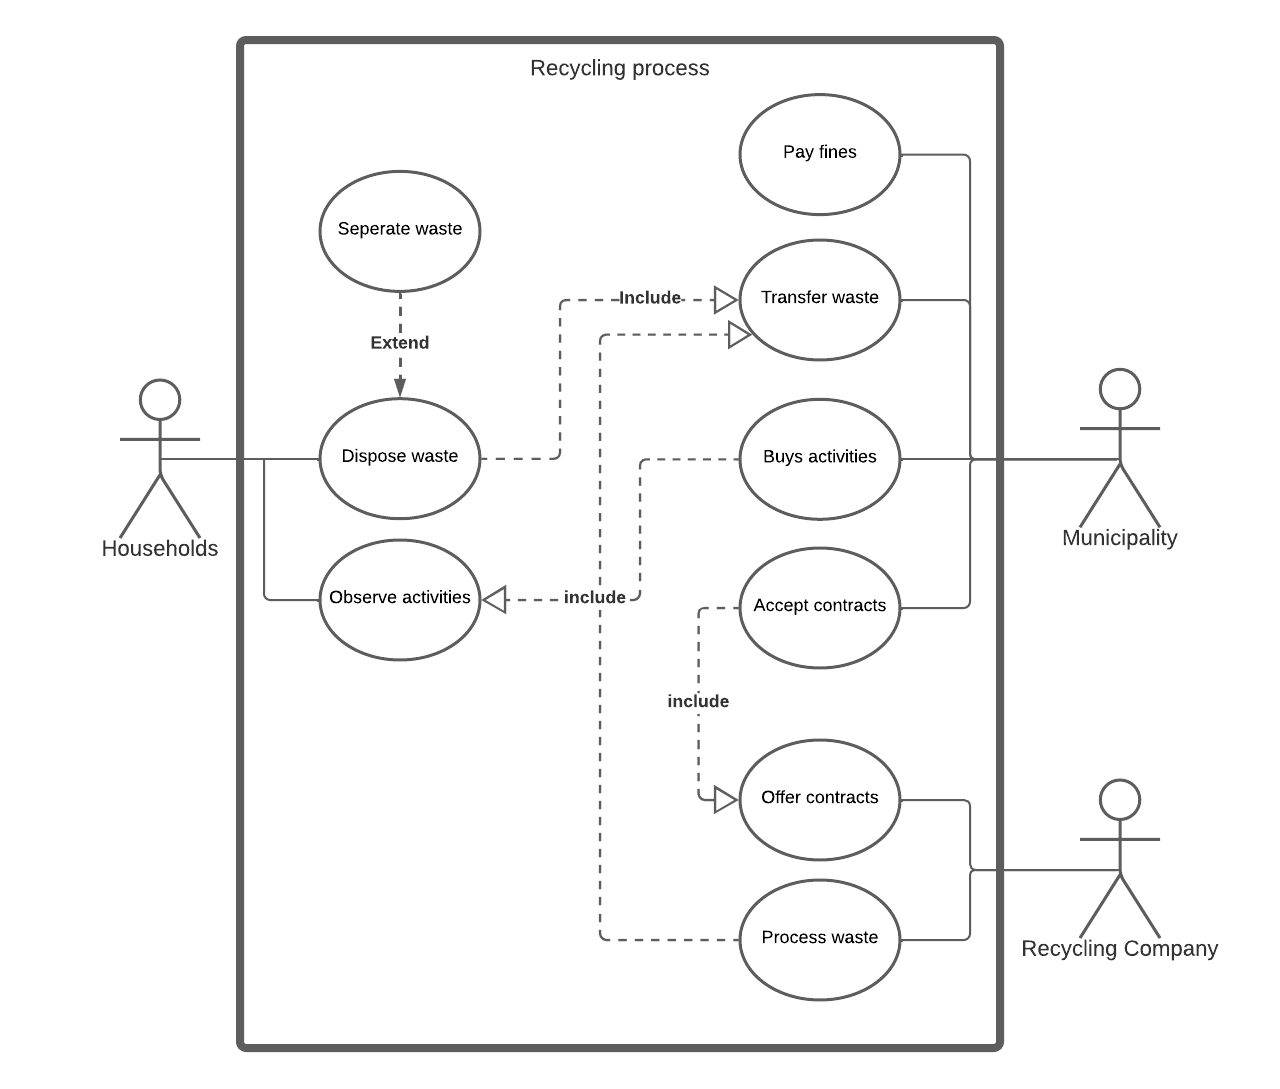
\includegraphics[width=0.95\linewidth]{Images/UML for recycling system - Use case (5).png}
        \caption{Use Case Diagram for waste recycling in municipality}
    \label{fig:Waste_Use_Case}
\end{figure}

\noindent Figure \ref{fig:Class-Diagram} provides an overview of the classes modelled for this research project. First, there is the agent classes. These classes includes the actual agents of the system and they are characterised by attributes (upper box) and actions or methods (lower box). An attribute is a variable value of the class. A method is an action the class can perform or undergo. Households consist of single, couple, elderly and Families. All share the same attributes and methods although values may differ. Their attributes define households' distance to a centralized waste disposal,  plastic production as well as their understanding, perception and importance in respect with recycling activities. Household agents are also able to perform actions: generating, separating and throwing out trash as well as being part of a policy activity.\\

\noindent The municipality also includes several attributes and methods. The municipality buys activities, has several waste contracts, recycling targets, budget, several attributes related to demographic information. 
The municipality's methods include choosing contracts, buying activities and paying fines.\\

\noindent The final agent is the recycling company. The attributes consist of active contracts, collected fines and technology. The recycling company is responsible for offering contracts, collecting waste and fining the municipality if the agreed amount of waste is not met.\\

\noindent Besides the agents, there are so-called 'non-agents'. These objects are: waste, contract, offer and activity.
\noindent Waste consists of the attribute Household data to track where the waste comes from. Waste can be generated and then transferred from households to the municipality. Contracts include more specifications such as the cost, the duration and how much plastics or waste is being collected. These contracts specify the quantity of plastic collected and the plastic recycling rate.\\

\noindent An offer is made of attributes such as the amount of trash, the potential fine, the target and the base waste foreseen in the contract.\\

\noindent The final class is the Activity. Activities can be implemented by the municipality to trigger change in the perception, knowledge and importance factor of the households or improve accessibility of collection points. The attributes of the activities combine the cost, effect per step, efficiency of the activity on the targeted variables, and the duration of the activity.

\begin{figure}[H]
    \centering
        \captionsetup{width=\linewidth}
        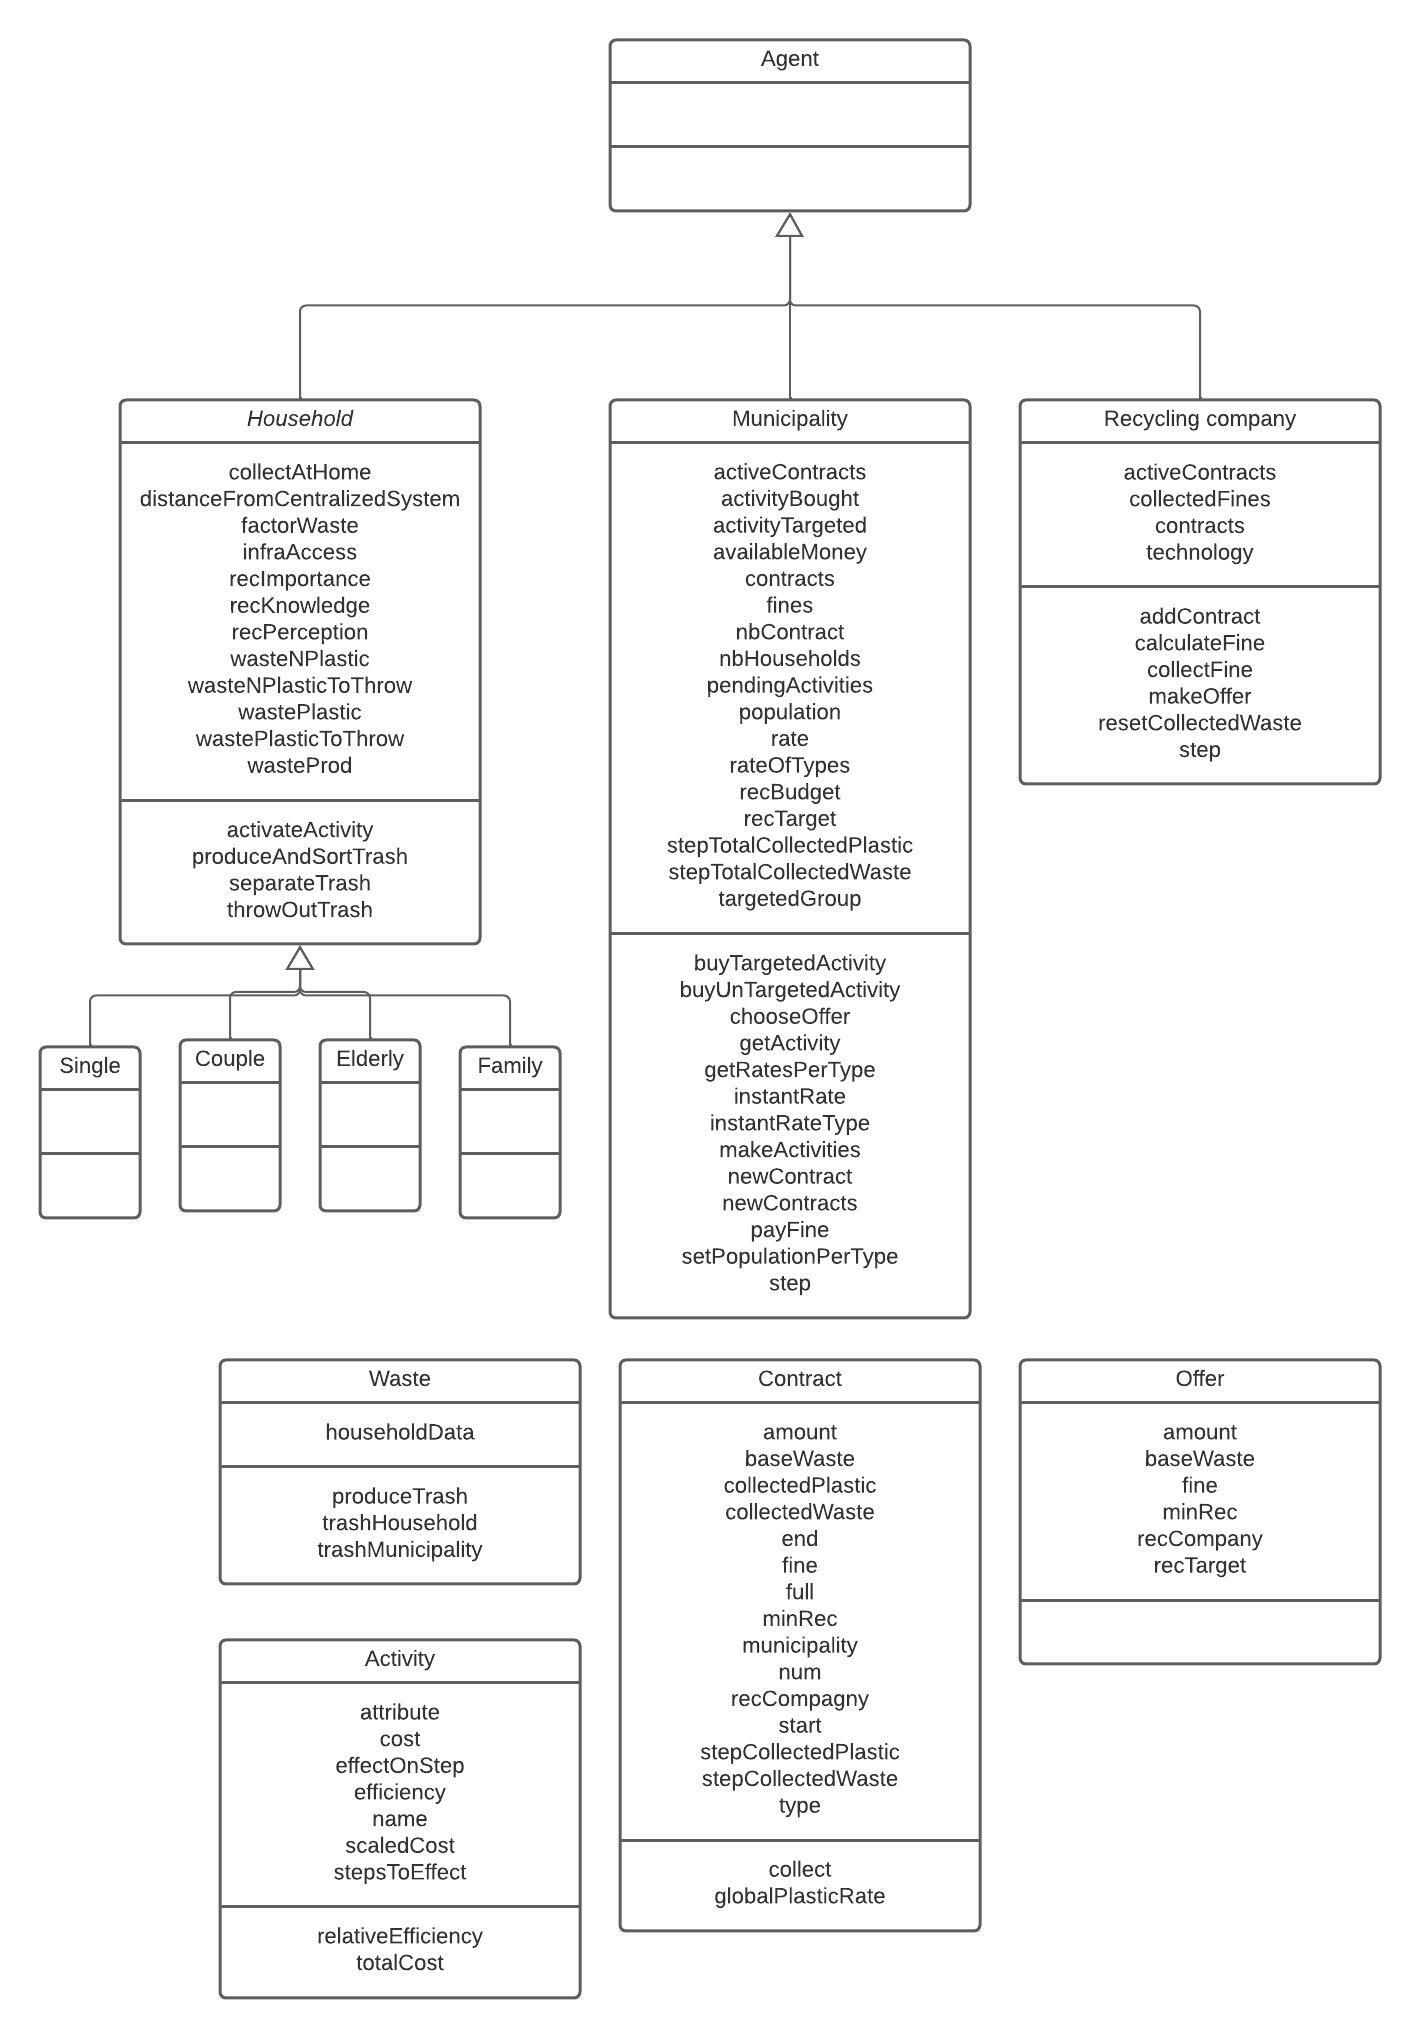
\includegraphics[width=1.0\linewidth]{Images/UML for recycling system - Pagina 3.jpeg}
        \caption{Class Diagram in the model}
    \label{fig:Class-Diagram}
\end{figure}

\subsection{Formal model and implementation}
\noindent In this subsection we will discuss the Formal model and its implementation in Python. The model was built using the mesa \cite{Mesa} framework in Python. The base Model class was extended to create the \textbf{RecyclingModel.py} class. This is the main model of the simulation and contains many agents extended from the Agent class from the mesa framework. These agents are of three different types: Municipality, Household or Recycling company. There are also classes for Contracts, Offers (of the contract), Activity and Waste. The model uses a slightly modified (local) version of the randomActivation Schedule. The model also has many data collectors which track many attributes during the execution of the code to give us our outputs.\\

\noindent Upon the creation of the agents, we use a normal distribution (defined by mean and standard deviation) to obtain the values of their attributes. In this sense we are able to create a large variety of agents that all have different values but who's values and the spread of these values is realistic.\\

\noindent Each Class contains many functions which we will not go in detail about as they are quite heavily commented and mostly self explanatory however the most important function is the step() function. This function is called every time a "time step" takes place in the code and launches a sequence of events which makes the model function and "live". We will now go in depth into this sequence of events and what happens in the code execution.
\newpage

\subsubsection{The step() function}

In this subsection we will discuss what each agent does at each step function.
\newline

The Municipality will do these things at each step: 
\begin{itemize}
    \item Archive ended contracts
    \item Buy new contracts if needed 
    \item Check the rate of recycling, if rate too low and end of year -> buy activity
\end{itemize}
\\
To buy an activity the municipality will: 
\begin{itemize}
    \item Check the rate of recycling for each type of household
    \item If the households recycle about the same --> buy most efficient activity for whole municipality
    \item Otherwise buy targeted activity for lowest performing type of household
\end{itemize}
\\
The Household will do these things at each step: 
\begin{itemize}
    \item Produce the trash
    \item Determine using its individual perception, knowledge and importance towards recycling how much of its plastic waste it will recycle
    \item Separate the trash based upon the above
    \item Throw out the trash in this manner either with at home collection or at a centralized collection spot
    \item Check for new activities 
    \item If new activity available from municipality then do it 
\end{itemize}
\\
Finally the recycling company at each step will: 
\begin{itemize}
    \item Reset the trash it collected at the previous step
    \item Collect the trash 
    \item If the contract is over Make offer for a new contract
\end{itemize}
\\
\noindent As can be seen above, the main functionality of the model is very simple but of course there is a lot more complexity that goes into it which can be seen from simply running the code in the debug function to go through an entire step. 

\newpage
\subsubsection{config.json file}

The \textbf{config.json} file  contains all the main variables for the model. Using such a file permitted us to avoid having dozens of hard coded variables spread all over the code and enabled a centralized file where all these variables were present. The \textbf{config.json} file is present below with a quick explanation of the purpose of each variable. 

\begin{verbatim}
{
  "households": {                       
    "family": {                         # object containing the values for the family household type
      "demographic" : 0.07,             # the % of households of this type in municipality
      "rateFactor" : 2.5,               # waste production as a factor of base
      "recPerception": {                # the perception towards recycling as a normal distribution
        "Mean": 0.5,
        "Var": 0.025
      },
      "recImportance": {                # the importance towards recycling as a normal distribution
        "Mean": 0.5,
        "Var": 0.075
      },
      "recKnowledge": {                 # the knowledge towards recycling as a normal distribution
        "Mean": 0.5,
        "Var": 0.025
      }
    }
    
    ... similar object as above for retired, couple, single ...
    
  },
  "lengthContract" : 3,                 # length of contract in years
  "nBContract": 5,                      # maximum amount of contracts extisting at once
  "moneyDispoPerHousehold": 1100,       # budget of municipality for each household for 20 years
  "recyclingTarget": 0.5,               # starting recycling target (50%)
  "pricePerTon": 30,                    # price of collecting 1 ton of waste in euros
  "plasticRateInWaste" : 0.195,         # Rate of plastic in waste (19.5% of waste is plastic)
  "distanceToCenter" : {                # How far a household is to collection spot (norm dist)
    "Min" : 30,
    "Mean" : 150,
    "Var" : 50,
    "Max" : 300
  },
  "fineFactor" : {                      # Variables used to determine how much a fine is 
    "factor" : 0.1,
    "delta" : 0.1
  },
  "partAtHome" : {                      # Uniform distribution of households having at home collection
    "Min" : 0.55,
    "Max" : 0.65
  },
  "contractTargetDelta" : 0.03,         # Variance in contract making on target
  "contractPriceDelta": 0.03,           # Variance in contract making on price
  "accessProportion" : {                # Uniform distribution of household access to infrastructure
    "Min" : 0.90,
    "Max" : 0.981
  },
  "numberOfHouseholds" : 1000,          # Total number of households in municipality
  "numberOfRecComps" : 10               # Total number of recycling companies in municipality
}
\end{verbatim}

\newpage 

\subsection{Verification and Validation}
\noindent After having introduced the formal model and explained its implementation in Mesa, this section describes the tests conducted to observe how the model behaves under various conditions ans so answering the first research question. With these verification runs, attributes' values are eventually validated to define a final model that delivers stable and acceptable results. For each run and the three scenarios, five indicators are analysed: (1) type and number of activities bought, (2) budget consumed, (3) waste and (4) plastic collected as well ass (5) plastic recycling rate. Based on observations, attributes' values are adapted to refine the model's output.\\

\subsubsection{Run 1 - Initial conditions:}
For the first verification run, figure \ref{fig:Run 1 activities} shows that the only activities bought are digital and billboard campaigns. New collection points are not built, either because the efficiency does not justify the construction cost (10.000€/collection point) or because the network of collection points has reached saturation. Saturation means here that adding new collection points does not improve the quantity of waste collected nor the recycling rate. Educative events foreseen by the municipality are not implemented either mainly because this activity does not sufficiently boost the perception, importance and knowledge of households regarding plastic recycling. 


\begin{figure}[H] 
    \centering
        \captionsetup{width=\linewidth}
        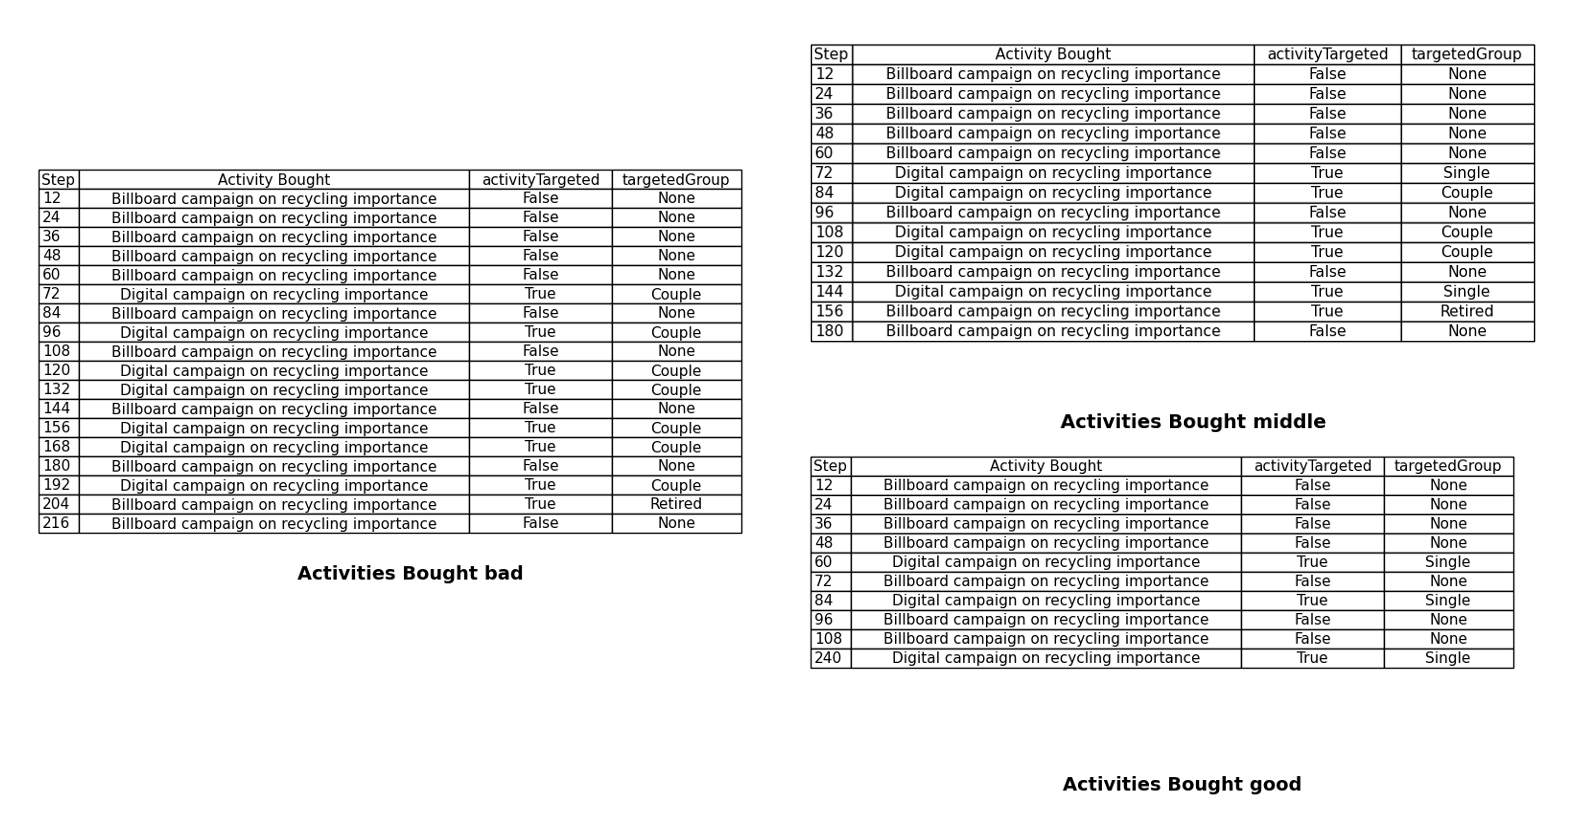
\includegraphics[width=1.0\linewidth]{Images/Run 1 Activities.png}
        \caption{Run 1: Activities bought for the bad, middle and good scenarios}
    \label{fig:Run 1 activities}
\end{figure}\\

\noindent As we can see in figure \ref{fig:Run 1 budget}, budget consumed in the three scenarios is almost the same. In addition no scenario uses a significant share of the budget available for plastic recycling although the bad scenario implements many more activities to reach the recycling target rate. The explanation can be found in the cost to run the activity. The activity cost is set per step and household. However, the budget per household for each activity has been estimated for the actual number of households in the municipality (48 177). However, the model runs with only 1000 households to speed the execution of the code. Therefore, the cost of activities should be multiplied by 50 to be aligned with the municipality's global budget.

\begin{figure}[H]
    \centering
        \captionsetup{width=\linewidth}
        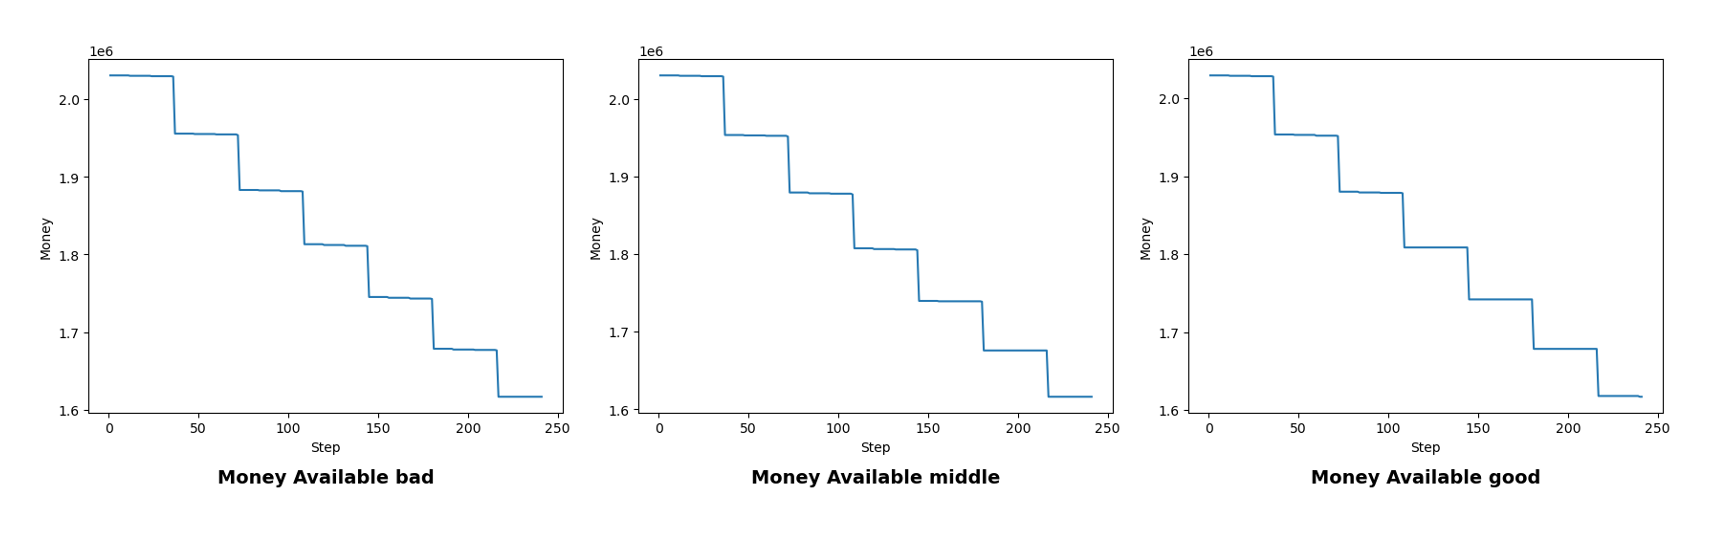
\includegraphics[width=1.0\linewidth]{Images/Run 1 budget.png}
        \caption{Run 1: Budget consumed for each scenario}
    \label{fig:Run 1 budget}
\end{figure}\\

\noindent Figures \ref{fig:Run 1 waste collected} and \ref{fig:Run 1 plastic collected} show that the quantity of waste and plastic collected experiences several drops with different magnitude for each scenario. These collection drops take place at the end of contracts with recycling companies. The issue in the model comes from the fact that households have the possibility to dispose trash in nearby municipal collection containers even if they can benefit from "at home" collection service. When the distance from home and the containers is smaller than 300m, households discard waste in containers rather than waiting for collection. This means that stock capacity in containers can be exceeded. Thus, the recycling company cannot cope with the quantity of waste gathered at collection points while little is being collected at home. Then, when a new contract starts, the newly appointed organisation must deal with a large amount of untreated waste. This is demonstrated in the graphs by the peaks in waste and plastic collected. This instability in the model must be addressed by defining stricter rules on the collection methods assigned to households.
\begin{figure}[H]
    \centering
        \captionsetup{width=\linewidth}
        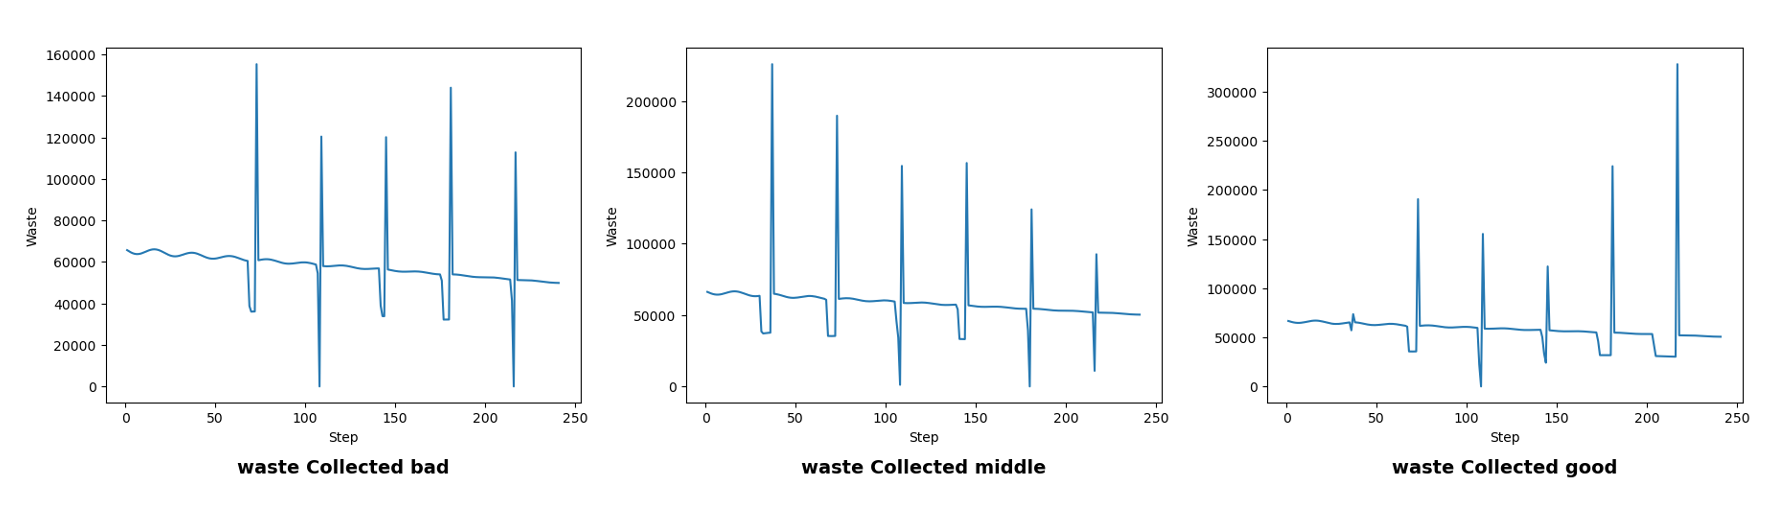
\includegraphics[width=1.0\linewidth]{Images/Run 1 waste collected.png}
        \caption{Run 1: Waste collected over time for each scenario}
    \label{fig:Run 1 waste collected}
\end{figure}

\begin{figure}[H]
    \centering
        \captionsetup{width=\linewidth}
        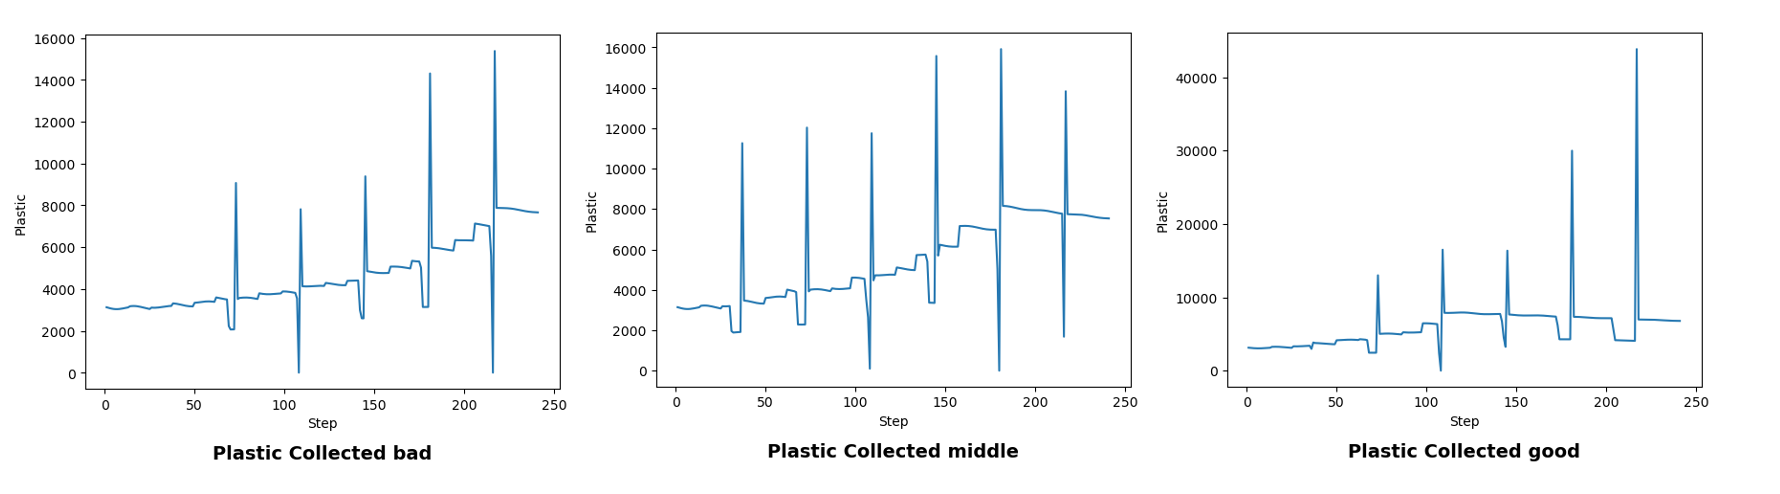
\includegraphics[width=1.0\linewidth]{Images/Run 1 plastic collected.png}
        \caption{Run 1: Plastic collected over time for each scenario}
    \label{fig:Run 1 plastic collected}
\end{figure}

\noindent Surprisingly, the recycling rate at the end of the 20-year period is higher for the bad and middle scenarios although they are expected to deliver weaker results. In addition, drops in the recycling rate (figure \ref{fig:Run 1 recycling rate}) observed for all scenarios remind us the drops seen in waste and plastic collection (figures \ref{fig:Run 1 waste collected} and \ref{fig:Run 1 plastic collected}). Addressing the drops in the collection of waste and plastic shall probably stabilise the recycling rate for all scenarios too. 

\begin{figure}[H]
    \centering
        \captionsetup{width=\linewidth}
        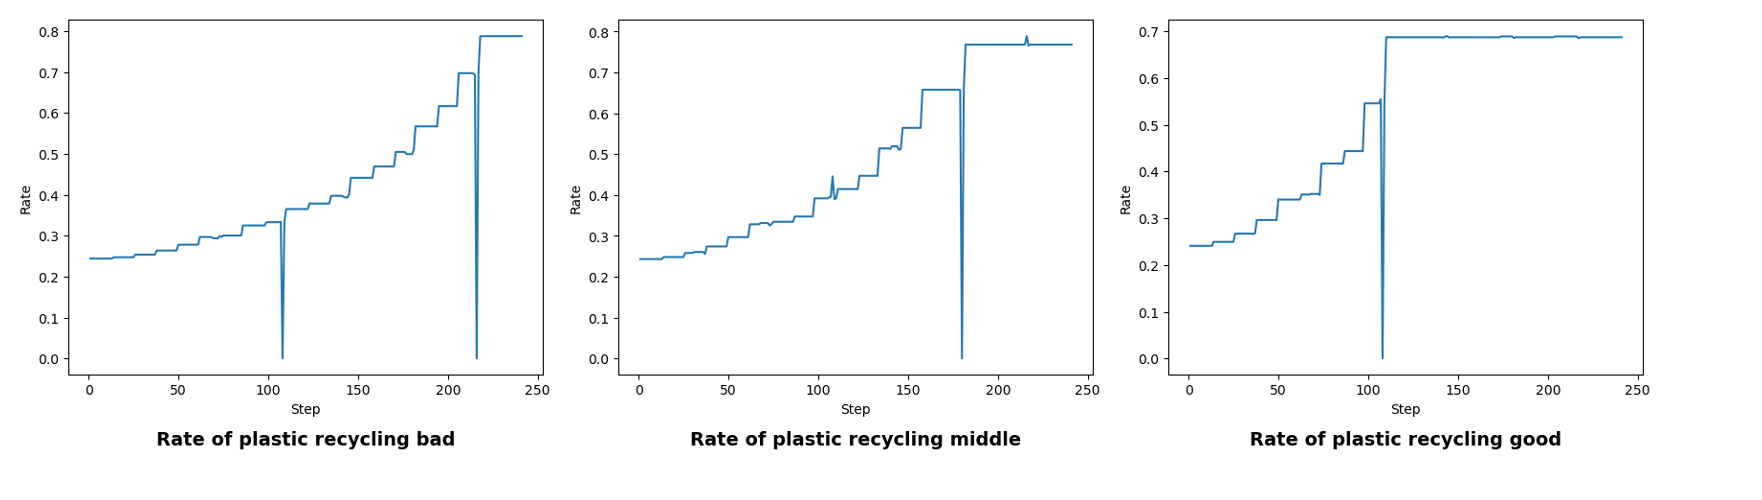
\includegraphics[width=1.0\linewidth]{Images/Run 1 recycling rate.png}
        \caption{Run 1: recycling rate for each scenario}
    \label{fig:Run 1 recycling rate}
\end{figure}\\

\subsubsection{Run 2 and 3 - New activity costs:}
We saw in the first verification run that budget available was underused. As explained, this issue came from the misalignment between the estimated activity cost per step and household and the number of households created in the model. To align the activity cost with the municipality's budget, the activity cost was first multiplied by 50. As we can see in figure \ref{fig:Run 2 budget}, the budget is more extensively consumed. Over the 2 million euros available, around 1 million is used for each scenario. In addition, the same figure shows that budget is not only consumed for staring new contracts but also for deploying billboard and digital campaigns neither as educative events nor new collection points are selected by the model. For the third, run, the activity cost was multiplied by 100 compared to the initial values. In addition, the cost of building new collection points was divided by two while keeping the same impact on the recycling rate. However, types of activities bought remained limited to billboard and digital campaigns. The budget graphs are not shared in this report because they demonstrate the same patterns as in figure \ref{fig:Run 2 budget}. The only difference is that the remaining budget at the end of the 20-year time frame for recycling activities drops to 0,4, 0,7 and 0,9 million euros respectively for the bad, middle and good scenario. Therefore, the initial budget of 2100€ foreseen per household for recycling activities over 20 years is too ambitious for the activities suggested in this model.\\

\subsubsection{Run 4 and 5 - rationalising the model :}
The fourth run consisted of reducing the budget per household dedicated to recycling activities from 2100 to 1100. Suggesting additional and bolder measures could have been an alternative to budget reduction. Due to time constraints, these model improvements could not be delivered. As explained in the next section "Simulation and data analysis", the main consequence is that budget is almost completely used after 20 years and the municipality may even run out of budget for some scenarios. \\

\noindent The final verification run was then launched to solve inconsistent waste and plastic collection scores as well as the related recycling rate as we observed in the first run. The model was stabilised by applying stricter rules on households' options for disposing trash. The method used is to set a fixed share of households that benefit from "at home" collection to dispose their waste in containers. This share ranges between 55 and 65 percent of the population. Consequently, collection points in neighbourhoods do not get overloaded and all trash disposed can be treated by the municipality. The outcomes of this modification in the model is more extensively presented in the last step of the modelling cycle: simulation and data analysis.

\begin{figure}[H]
    \centering
        \captionsetup{width=\linewidth}
        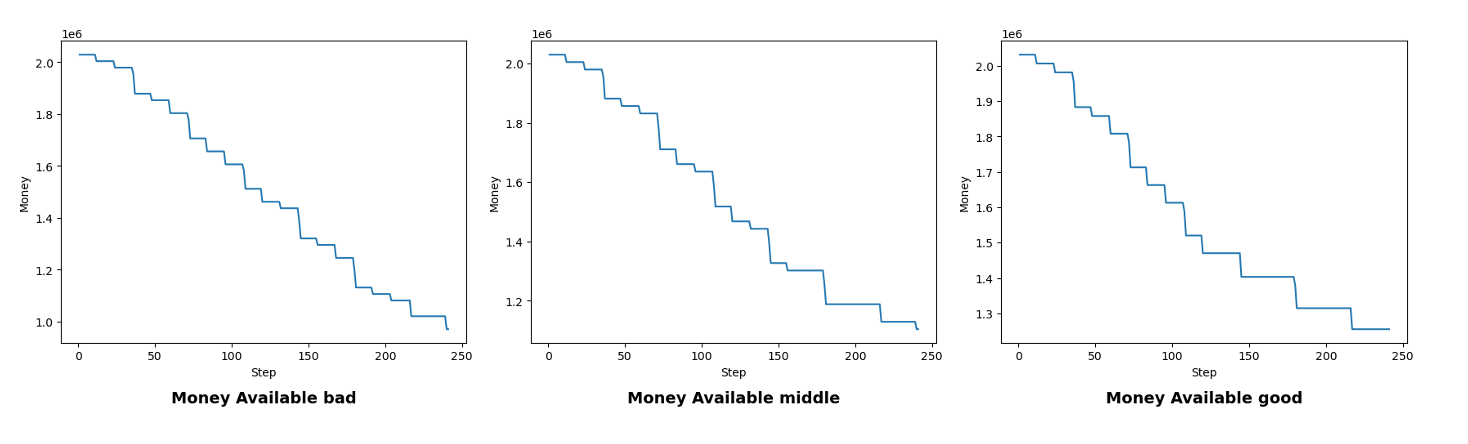
\includegraphics[width=1.0\linewidth]{Images/Run 2 budget.png}
        \caption{Run 2: Budget consumed for each scenario}
    \label{fig:Run 2 budget}
\end{figure}\\

\noindent To conclude this section and summarise our answer to the first research question, we observed that the choice and frequency of activities implemented are not strongly sensitive to changes in cost. The number of policies launched over 20 years remained stable across the five verification runs. However, the budget available for policy measures is naturally affect by these changes in cost. Another key finding is that preventing households benefiting from "at home collection" to dispose trash in containers, allows the municipality to better control the waste flows and so better manage collection. The next section of the modelling cycle describes the simulation settings of the final model and the analysis of its output.  

\newpage
\subsection{Simulation and Data Analysis}
The simulation and data analysis section is the last piece of the modelling cycle. This part presents the results of the final model that must support the municipality's future decisions to boost the plastic recycling rate in its area. The model's output are analysed according the five key indicators listed in the previous section. 

\subsubsection{Activities}
\noindent The first indicator to be analysed is the types of activities bought by the municipality. \\

\noindent Figure \ref{fig:Activity_tables} shows that an activity is bought every year. In the middle scenario the municipality bought yearly activities for 15 years (up to step 180). In the good scenario, the municipality launched yearly activities for 10 years (up to step 120) and then implemented an additional activity for the 15th year (from 180 to step 191 included) of the model. The reason for this becomes clear when analysing results from the following subsections. In principle, the municipality stops buying activities when the recycling target are met. The recycling target starts in year one with the objective to increase by 5 percent every four years. In the bad scenario, activities bought never achieve the reach the recycling target. In the middle scenario, the target seems to be met after 15 years (step 180). Then the municipality stops buying activities from this moment onward. In the good scenario the target is met during the 10th year of the model. However, the municipality starts a new campaign in year 15 to maintain the recycling rate after a five-year period without buying activities. \\

\noindent Besides the amount of activities bought, some of the activities are targeted at a specific group. First the model analysis if there is a specific group which has an outlying recycling rate. If this is the case, an activity is bought which has the most impact on that group. We observe that campaigns are either targeted to all household types or to elderly people. This is caused by the fact that digital campaigns focus on all demographic groups except elderly since those people are less affected by those types of campaigns. After a implementing a digital campaign, the perception, knowledge and importance of recycling are improved with billboard campaigns. This phenomena can be seen in all three scenarios.

\begin{figure}[H]
    \centering
        \captionsetup{width=\linewidth}
        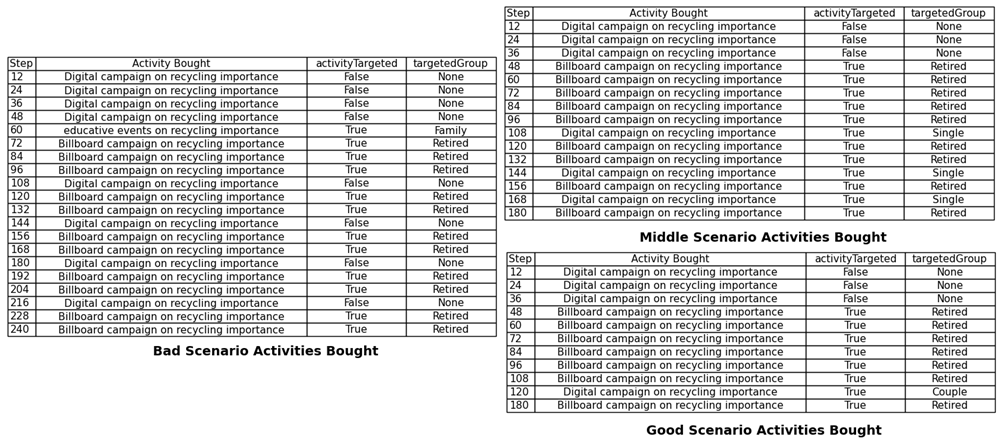
\includegraphics[width=1.0\linewidth]{Images/Activity_tables.png}
        \caption{Lists of bought activities for the three scenarios}
    \label{fig:Activity_tables}
\end{figure}

\subsubsection{Budget}
\noindent The second indicator tracks hows the budget is consumed through the years by buying activities and new contracts with recycling companies. \\

\noindent The municipality starts with a budget of 1100 euro per household for the next 20 years. The total budget for 1000 households reaches 1.1 million euros. To start of with the bad scenario, in the first graph of figure \ref{fig:Budget_graph} there can be observed that the budget moves down in a pattern. First there are 3 little jumps down, followed by a bigger step. This pattern repeats until the budget gets close to 0. Every year there can be one activity bought, and once every 3 years the municipality buys a contract. In the bad scenario, an activity is bought every year (see figure \ref{fig:Activity_tables}). This explains the repeating pattern in this scenario. The pattern found in the bad scenario was also visible in the middle and good scenario, but stops respectively after step 15 (step 180) and 10 years (120). As explained above, this is due to the municipality stopping to regularly launch new activities. Consequently, the municipality run out of budget only in the bad scenario. \\

\begin{figure}[H]
    \centering
        \captionsetup{width=\linewidth}
        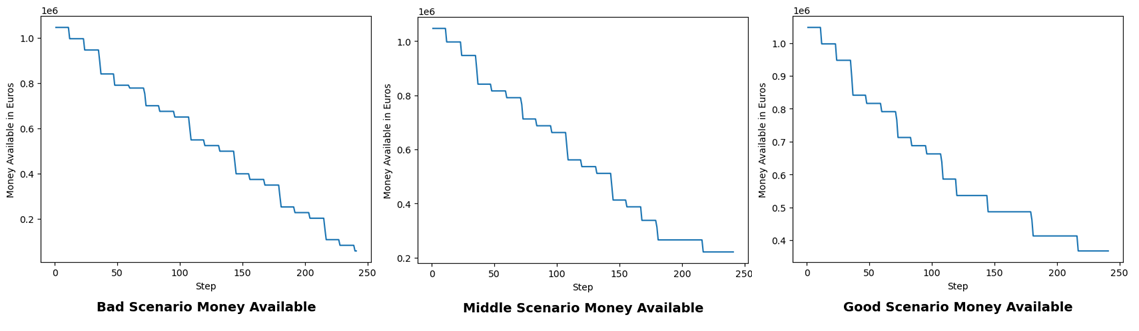
\includegraphics[width=1.0\linewidth]{Images/Budget_graphs.png}
        \caption{Budget consumed for the three scenarios}
    \label{fig:Budget_graph}
\end{figure}

\subsubsection{Waste collected}
\noindent In this subsection the third indicator is analysed: amount of collected waste. \\

\noindent From figure \ref{fig:Waste_collected_Graph} it can be concluded that the amount of waste collected stays approximately the same over the 3 different scenarios. The periodically fluctuations are caused by the waste production function given in the assignment. The middle scenario however shows a slight decrease in the amount of waste collected from the start. This indicates that the amount of waste produced is slightly lower in the scenario. 

\begin{figure}[H]
    \centering
        \captionsetup{width=\linewidth}
        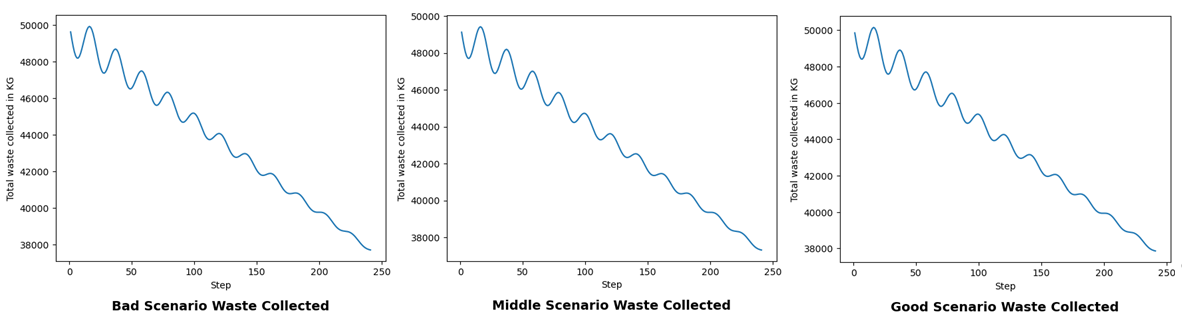
\includegraphics[width=1.0\linewidth]{Images/Collected_waste_graphs.png}
        \caption{}
    \label{fig:Waste_collected_Graph}
\end{figure}

\subsubsection{Plastic collected}
\noindent The fourth indicator analysed here focuses on the quantity of plastic collected. \\

\noindent The graphs in figure \ref{fig:Plastic_collected} show the that amount of plastic collected increases over time. In the bad, middle and good scenarios the maximum amount of plastic collected respectively exceeds  5000kg, 6000kg and 6100kg. When looking back at figure \ref{fig:Activity_tables}, we observe that the bad scenario needs activities every year. In addition we observe in \ref{fig:Budget_graph} that the budget is running out. These observations combined explain why in the bad scenario the total amount of plastic recycled is lower than in the middle scenario. In the middle scenario the peak is at step 180, where according to figure \ref{fig:Activity_tables} the last activity was bought. From this point, the graph continuously follows the waste production function provided in the assignment. In the good scenario, the first peak occurs at step 120, where the periodically activities stops. The final peak is at step 180, where the final activity is bought. These observations show the role played by activities increasing and maintaining the quantity of plastic collected for entering the recycling process. 

\begin{figure}[H]
    \centering
        \captionsetup{width=\linewidth}
        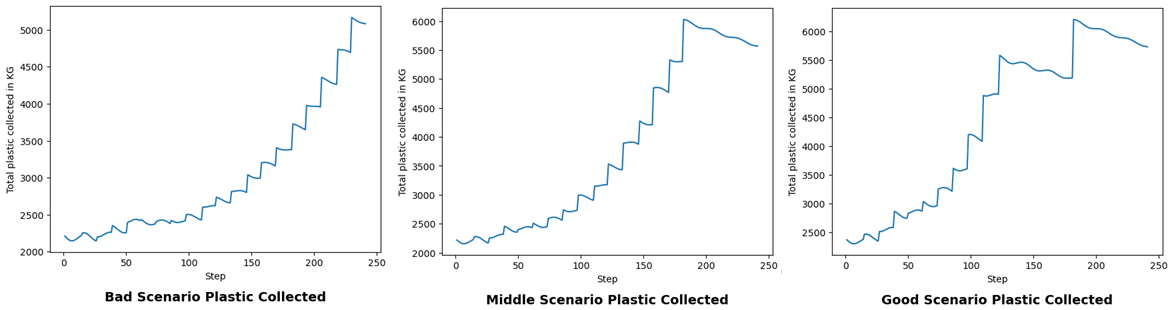
\includegraphics[width=1.0\linewidth]{Images/Collected_plastic_graphs.png}
        \caption{}
    \label{fig:Plastic_collected}
\end{figure}

\subsubsection{Recycling rate}
\noindent Finally, the analysis parts concludes with the plastic recycling rate obtained from the model. 

\noindent In figure \ref{fig:Recycling_rate_plastic} the recycling rate of the 3 scenarios are displayed. The goal of the model is to reach a recycling percentage of 50\%, increased by 5\% every 5 years. In the bad scenario this goal is never met. The recycling rate of plastic never reaches the intermediary steps and caps below the 70\% after 20 years. This explains the results from figure \ref{fig:Activity_tables} which shows that in the bad scenario the activities are bought every year, trying to catch up to the goal. In the middle scenario, figure \ref{fig:Recycling_rate_plastic} shows that the goal is met at step 180. This explains why the municipality stops buying activities at step 180, where the recycling rate peaks. Then, no additional activities must be launched because the recycling rate remains above target. In the good scenario, the goal is first met at step 120, where the goal was to have a recycling rate of 60\%. When suddenly after step 180 the goal increases to 65\%, it needs to buy another activity to increase its recycling rate. This explains why in figure \ref{fig:Activity_tables} the purchases of activities stops at step 120, and it explains why at step 180 another activity is bought. This also explains the 2 peaks in figure \ref{fig:Plastic_collected}, where at step 120 and 180 peaks are visible. 

\begin{figure}[H]
    \centering
        \captionsetup{width=\linewidth}
        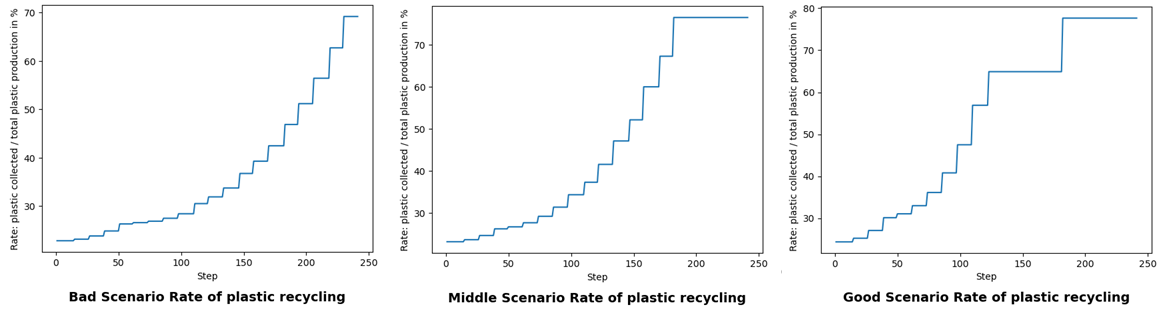
\includegraphics[width=1.0\linewidth]{Images/Recyclingrate_plastic_graphs.png}
        \caption{}
    \label{fig:Recycling_rate_plastic}
\end{figure}